\documentclass[handout]{beamer}
%\documentclass{beamer}
\mode<presentation> {%
	\usetheme[]{Boadilla}
	\usecolortheme{orchid}
	\setbeamercovered{transparent}
	\setbeamersize{text margin left=0.7cm}
  \setbeamersize{text margin right=0.7cm}
  \setbeamertemplate{enumerate item}[square]
  \setbeamertemplate{enumerate subitem}[circle]
  \setbeamertemplate{enumerate subsubitem}[>]
  \setbeamertemplate{itemize item}[square]
  \setbeamertemplate{itemize subitem}[circle]
  \setbeamertemplate{itemize subsubitem}[>]
}

% \usepackage{bm}
\usepackage[utf8]{inputenc}
\usepackage[spanish]{babel}
% \usepackage[normalem]{ulem}
% \usepackage{times}
% \usepackage[T1]{fontenc}
\usepackage{graphicx}
% \usepackage{multirow}
% \usepackage{rotating}
% \usepackage{colortbl}
% \usepackage{verbatim}
\usepackage{hyperref}
\hypersetup{colorlinks=true,linkcolor=blue,urlcolor=blue}
\usepackage{tikz}
\usetikzlibrary{shapes.geometric, arrows, positioning}
\tikzstyle{block} = [rectangle, draw, text centered, rounded corners, minimum height=2em, align=center]
\tikzstyle{arrow} = [thick,->,>=stealth]

\definecolor{olivegreen}{rgb}{0.0,0.5,0.0}
\definecolor{general}{rgb}{0.9 0.9 1}%

\title[Procesamiento de Señales]{Muestreo y reconstrucción de señales \\ en el dominio del tiempo}
\author[Jesús Chacón] {%
	\textit{Ingeniería Electrónica de Comunicaciones}\\
	\vspace{0.6cm}
	\small Jesús Chacón Sombría%
}%\inst{1}

\institute[DACYA] {%\inst{1}%
	\footnotesize  Departamento de Arquitectura de Computadores y Automática\\
  Universidad Complutense de Madrid
}

\date[Muestreo y reconstrucción] % (optional)
{\footnotesize Curso 2025-2026}%{\today / Master}
\subject{Talks}

\pgfdeclareimage[height=0.75cm]{logo}{ucm}

\usepackage[absolute,overlay]{textpos}
\setlength{\TPHorizModule}{1mm}
\setlength{\TPVertModule}{1mm}
\newcommand{\MyLogo}{%
\begin{textblock}{14}(116.0,0.6)
  \pgfuseimage{logo}
\end{textblock}
}

\makeatletter
\numberwithin{section}{part}
\AtBeginPart{
\beamer@tocsectionnumber=0\relax
\frame{\partpage}
}
\makeatother

\begin{document}

\begin{frame}
  \titlepage
\end{frame}

\newcommand*\oldmacro{}%
\let\oldmacro\insertshorttitle%
\renewcommand*\insertshorttitle{%
 \MyLogo
  \oldmacro\hfill%
}

\AtBeginSection[]{}
\AtBeginSubsection[]{}

\section{Objetivos}
\section{Conversión analógico-digital y digital-analógico}
\section{Muestreo de señales continuas}
\subsection{Muestreo periódico}
\subsection{Teorema del muestreo}

  \begin{frame}\frametitle{Efecto del muestreo periódico}
    {\tiny La transformada de Fourier se escala y se replica: $X_d(\omega)=\frac{1}{T_s}\substack{\infty\\\sum\\k=-\infty}X(\omega-\frac{2\pi}{T_s}k)$}
    \begin{center}
      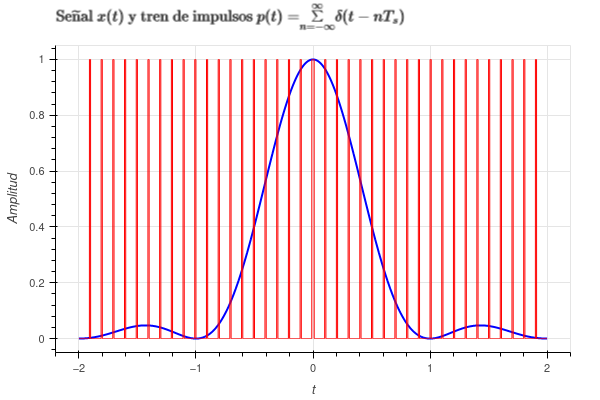
\includegraphics[width=3.5cm,clip,trim={0 0 0 30}]{Figures/sinc_1.png}
      \hspace{1cm}
      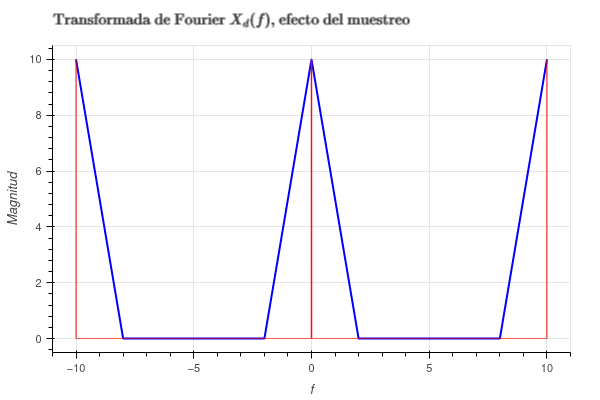
\includegraphics[width=3.5cm,clip,trim={0 0 0 30}]{Figures/muestreo_1.png}
      \\
      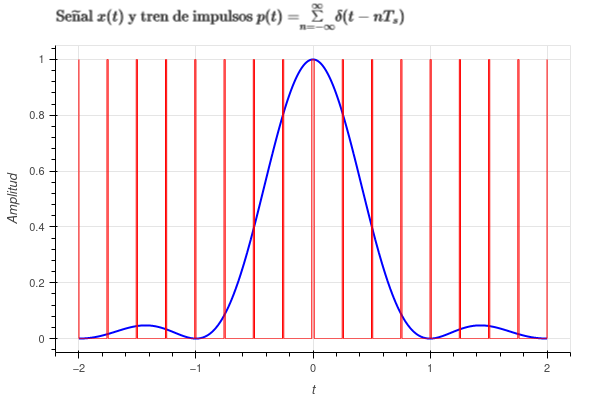
\includegraphics[width=3.5cm,clip,trim={0 0 0 30}]{Figures/sinc_2.png}
      \hspace{1cm}
      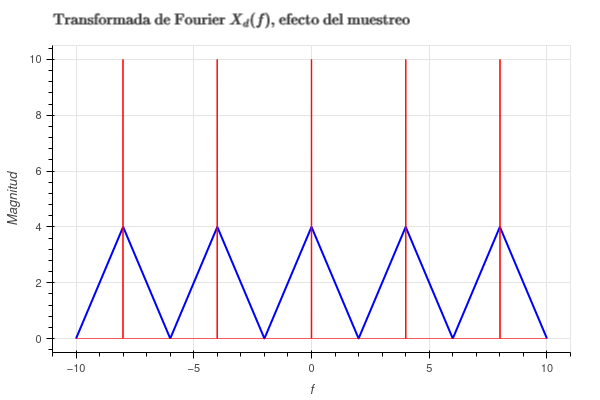
\includegraphics[width=3.5cm,clip,trim={0 0 0 30}]{Figures/muestreo_2.png}
      \\
      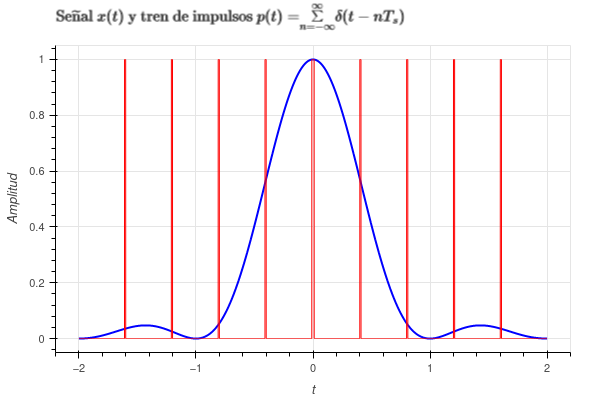
\includegraphics[width=3.5cm,clip,trim={0 0 0 30}]{Figures/sinc_3.png}
      \hspace{1cm}
      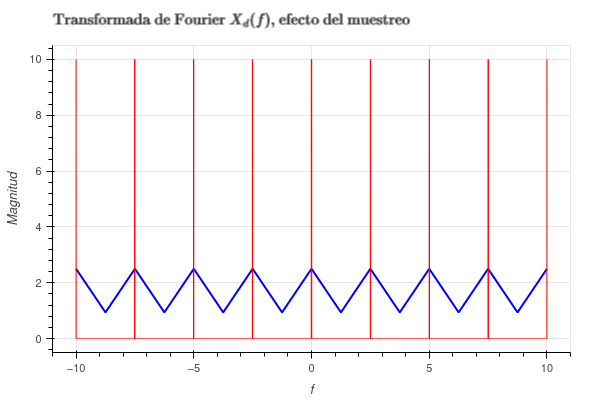
\includegraphics[width=3.5cm,clip,trim={0 0 0 30}]{Figures/muestreo_3.png}
    \end{center}
  \end{frame}

  \begin{frame}\frametitle{Teorema del muestreo}
    \begin{itemize}\footnotesize
      \item Señal $x(t)$ de ancho de banda $\omega_m$ limitado: \color{blue}$X(\omega)=0$ para $|\omega|>\omega_m$\color{black}.
      \item Al aumentar \color{blue}$T_s$ \color{black} la distancia entre copias disminuye \color{blue}($\omega_s=2\pi f_s= \frac{2\pi}{T_s}$)\color{black}
      \item Cada copia $k$ ocupa \color{blue}$k\omega_s-\omega_m\leq\omega\leq k\omega_s+\omega_m$\color{black}.
      \item En particular, $\omega\leq\omega_m$ y $\omega\geq\omega_s-\omega_m$ para $k=0,1$.
      \item En el límite para que no haya solapamiento, \color{blue}$\omega_m = \omega_s - \omega_m$\color{black}.
    \end{itemize}
    \begin{center}
      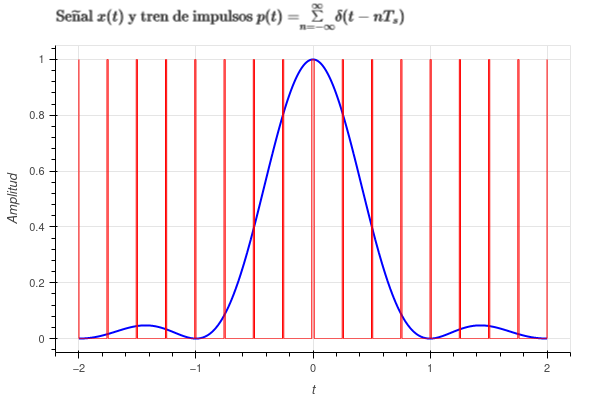
\includegraphics[width=5cm,clip,trim={0 0 0 30}]{Figures/sinc_2.png}
      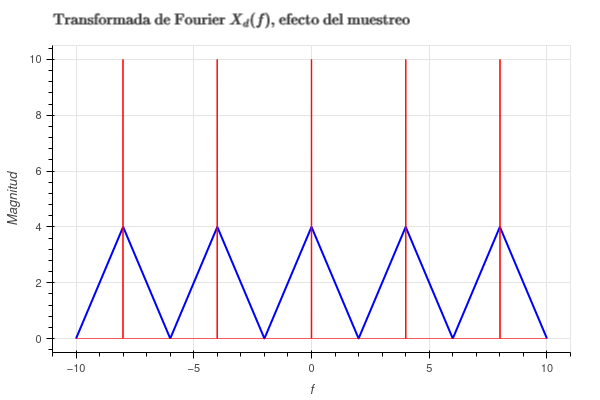
\includegraphics[width=5cm,clip,trim={0 0 0 30}]{Figures/muestreo_2.png}
    \end{center}
    \begin{alertblock}{Teorema del muestreo (Nyquist-Shannon)}
      Para que se pueda reconstruir una señal, es necesario que:
      \begin{itemize}
        \item la señal tenga ancho de banda limitado, $\omega_m$.
        \item la frecuencia de muestreo cumpla $\omega_s > 2 \omega_m$.
      \end{itemize}
    \end{alertblock}
  \end{frame}

  \begin{frame}\frametitle{Reconstrucción de señales}
    \begin{center}
      \raisebox{-.5\height}{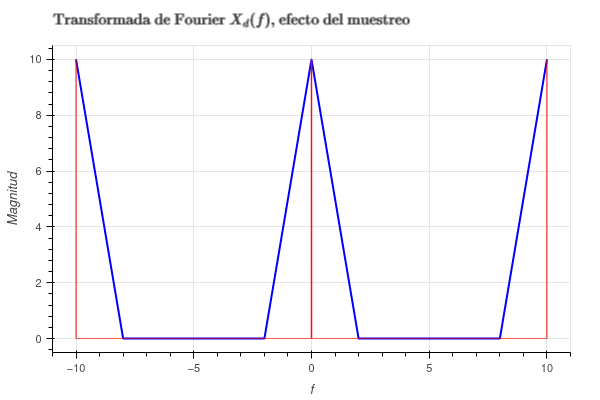
\includegraphics[width=6cm,clip,trim={0 0 0 30}]{Figures/muestreo_1.png}}
      \Huge $\leftrightarrow~?$
    \end{center}
    \begin{itemize}
      \item Suponemos que $x(t)$ ha sido muestreada con un $\omega_s$ adecuado.
      \item Recordemos que \color{blue}$X_d(\omega)=\frac{1}{T_s}\substack{\infty\\\sum\\k=-\infty}X(\omega-\frac{2\pi}{T_s}k)$\color{black}.
      \item Cada \emph{copia} es idéntica a la original, salvo por el escalado $\frac{1}{T_s}$.
    \end{itemize}
  \end{frame}

  \begin{frame}\frametitle{Reconstrucción de señales}
    \begin{center}
      \raisebox{-.5\height}{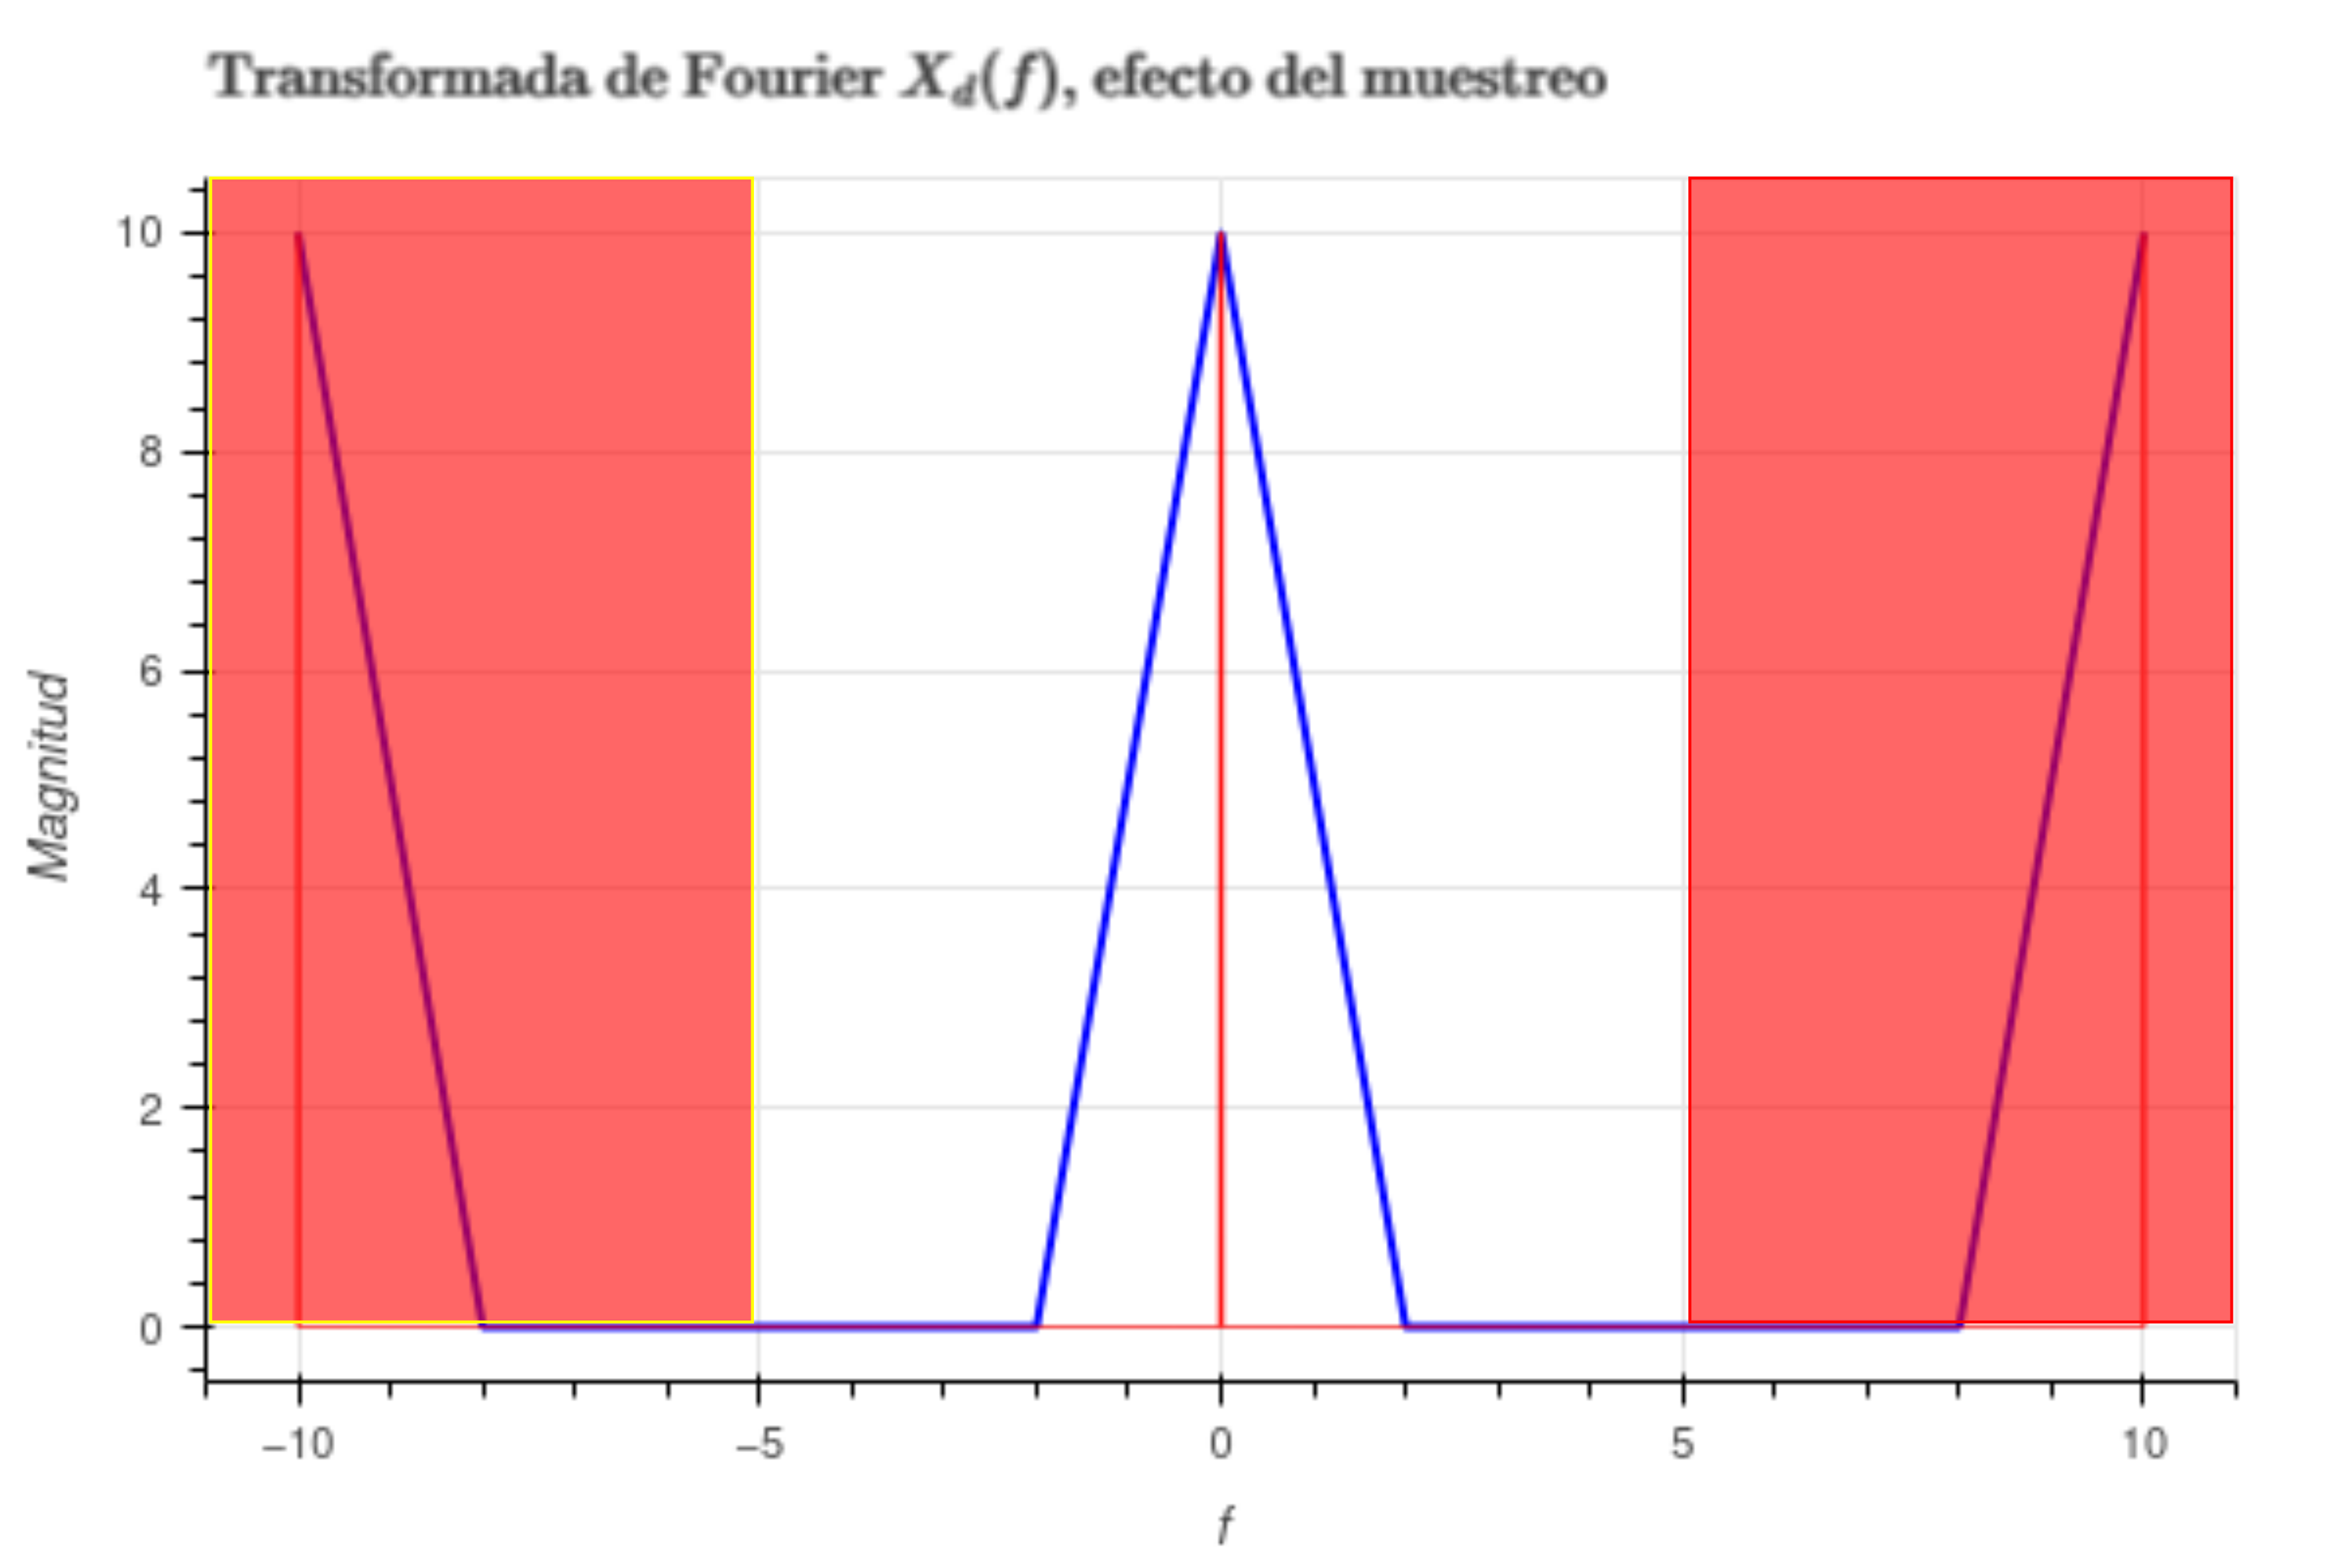
\includegraphics[width=6cm,clip,trim={0 0 0 22}]{Figures/reconstruccion_1.png}}
      \Huge $\leftrightarrow~?$
    \end{center}
    \begin{itemize}
      \item Podemos ''quedarnos una copia'' y descartar las demás.
      \item Más formalmente, lo que estamos haciendo es un filtro paso bajo.
    \end{itemize}
  \end{frame}

  \begin{frame}\frametitle{Reconstrucción de señales}
    \begin{center}
      \alert {Reconstrucción ideal}\\
      \raisebox{-.5\height}{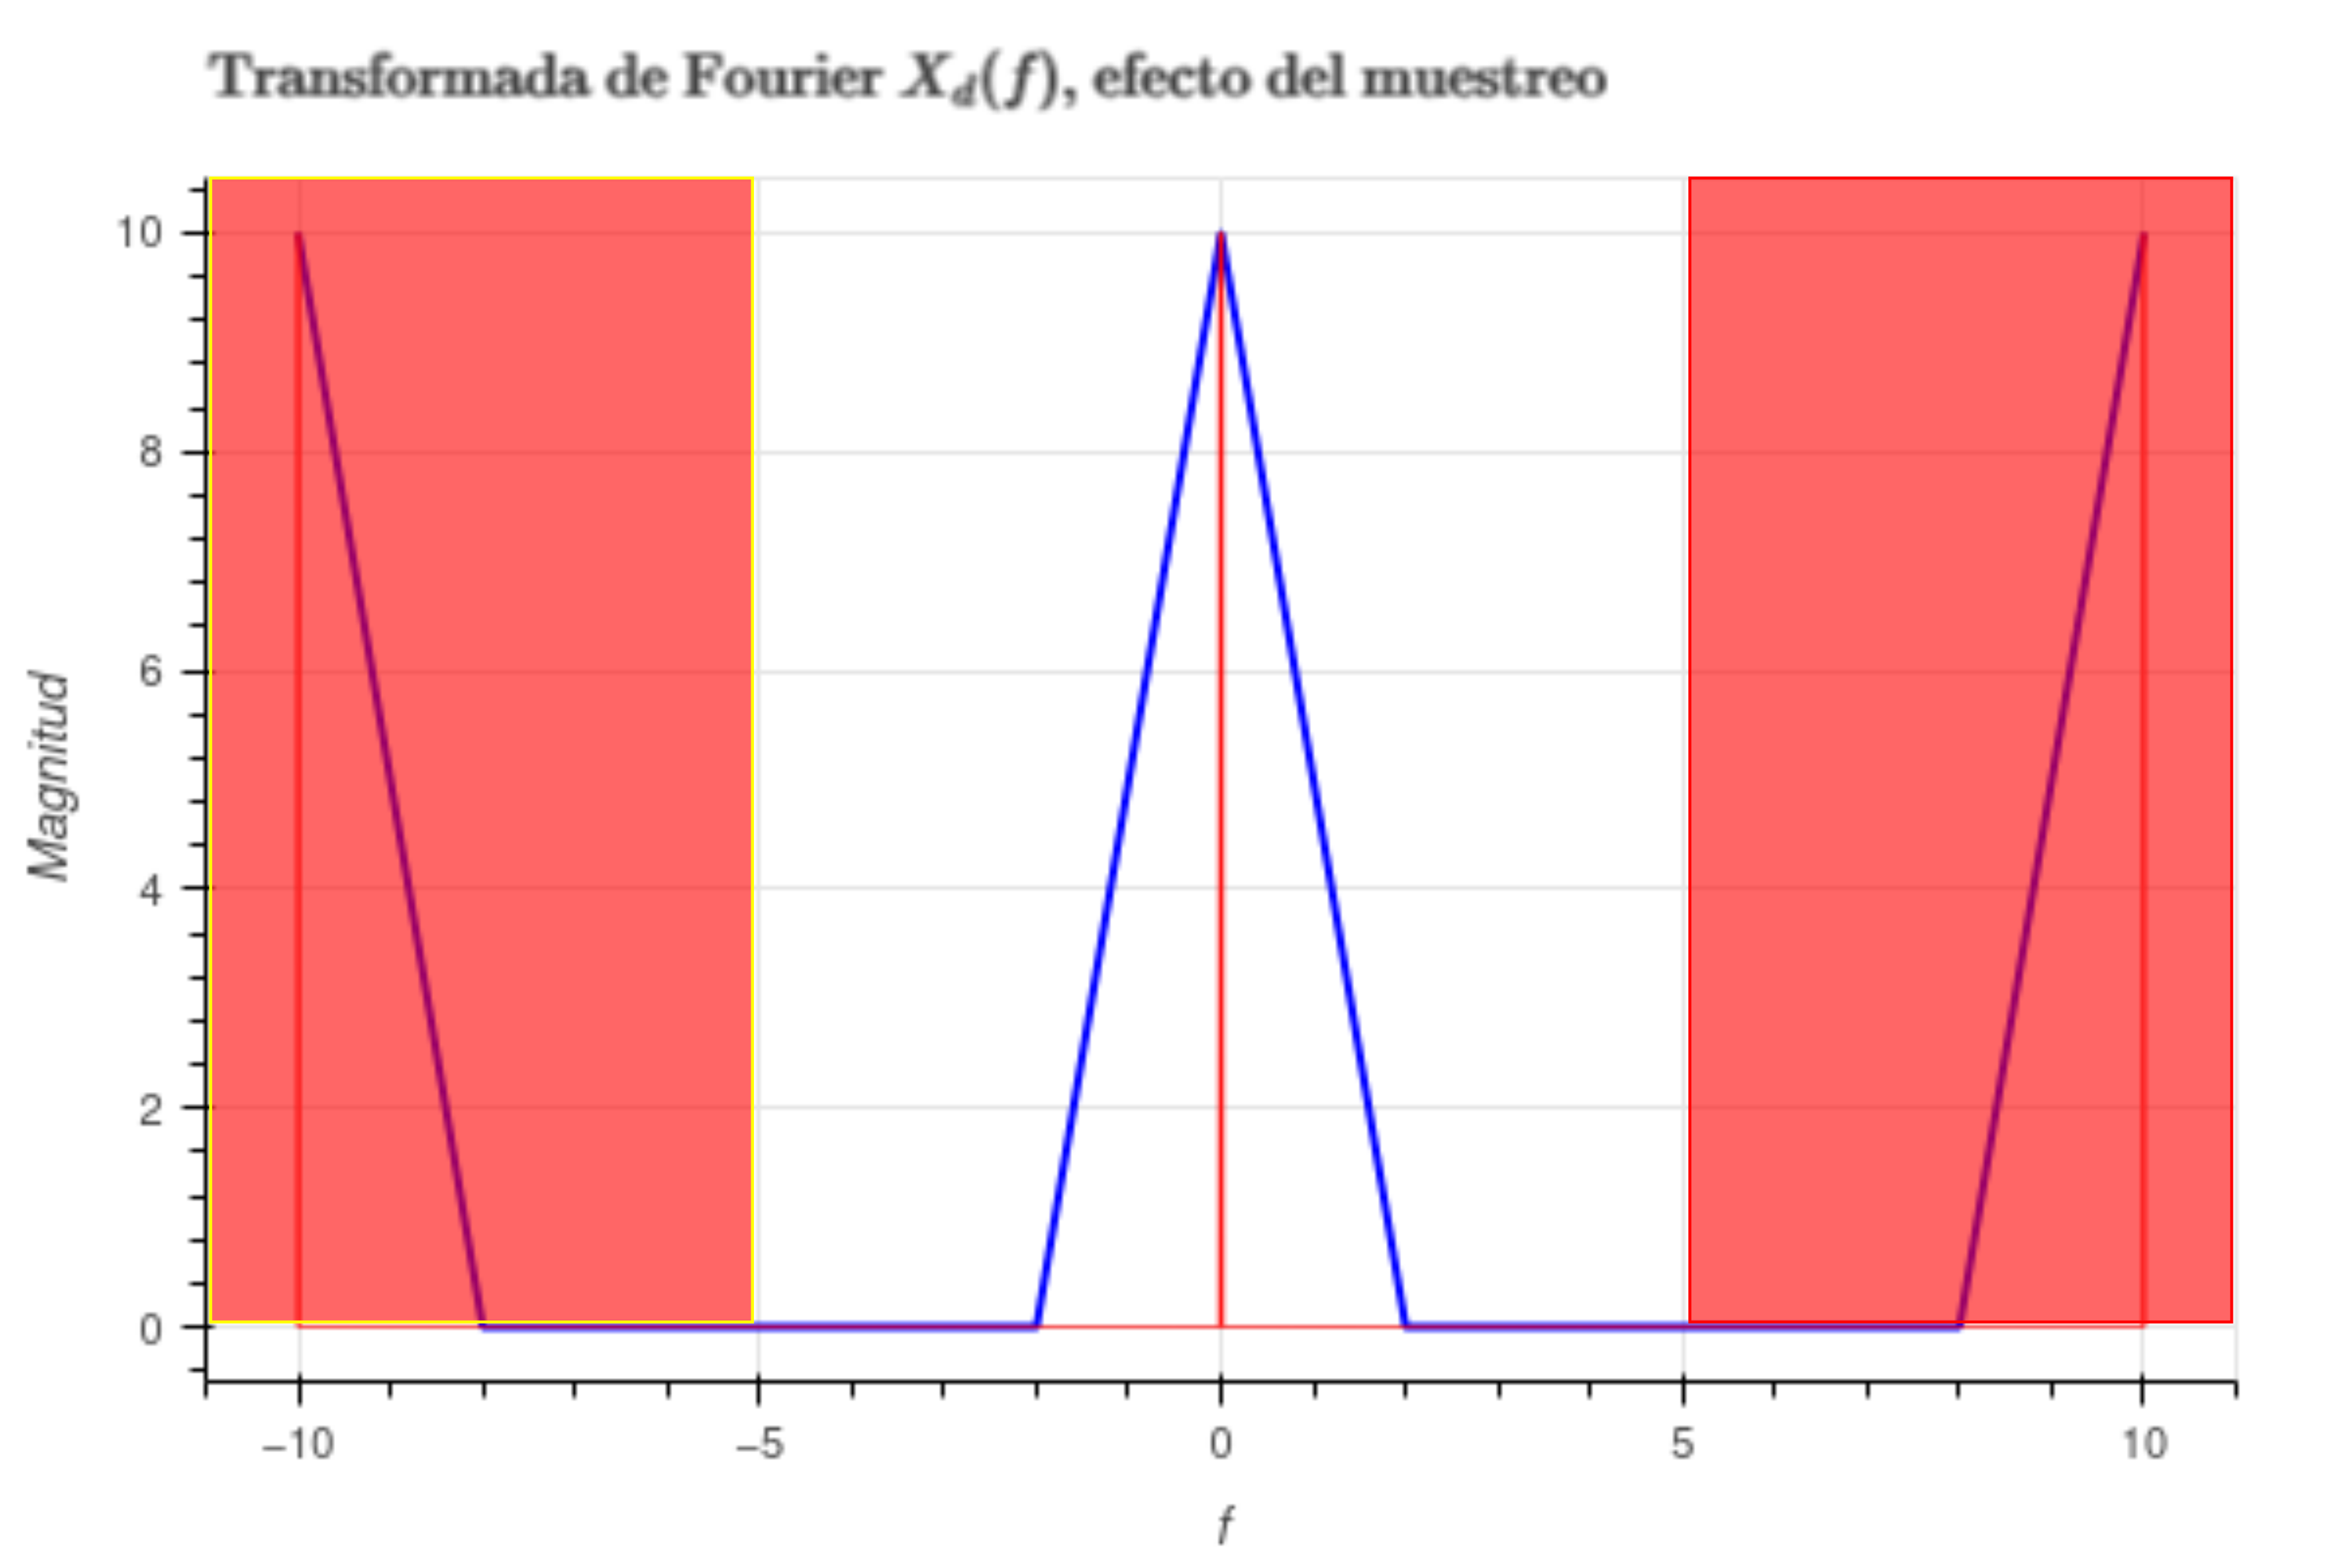
\includegraphics[width=5cm,clip,trim={0 0 0 22}]{Figures/reconstruccion_1.png}}
    \end{center}
    \begin{itemize}\small
      \item Utilizamos un filtro ideal: $H(\omega)=\begin{cases}T_s\phantom{0}~\text{si}~|\omega|\leq\omega_c\\0\phantom{T_s}~\text{si}~|\omega|>\omega_c\end{cases}$
      \item $T_s$ aparece para compensar el escalado inducido por el muestreo.
      \item Entonces, $h(t)=\frac{T_s}{2\pi}\int_{-\omega_c}^{\omega_c}\text{e}^{j\omega t}dt=\frac{\omega_c T_s}{\pi}\frac{\text{e}^{j\omega_c t}-\text{e}^{-j\omega_c t}}{2j\omega_c t}$\\
    \end{itemize}
    \begin{alertblock}{Respuesta impulso del filtro ideal}\centering
      $h(t)=\frac{\omega_c T_s}{\pi} \text{sa}(\omega_c t)=2 f_c T_s \text{sinc}(2 f_c t)$
    \end{alertblock}
  \end{frame}

  \begin{frame}\frametitle{Reconstrucción de señales}
    \begin{center}
      \alert {Reconstrucción ideal}\\
      \raisebox{-.5\height}{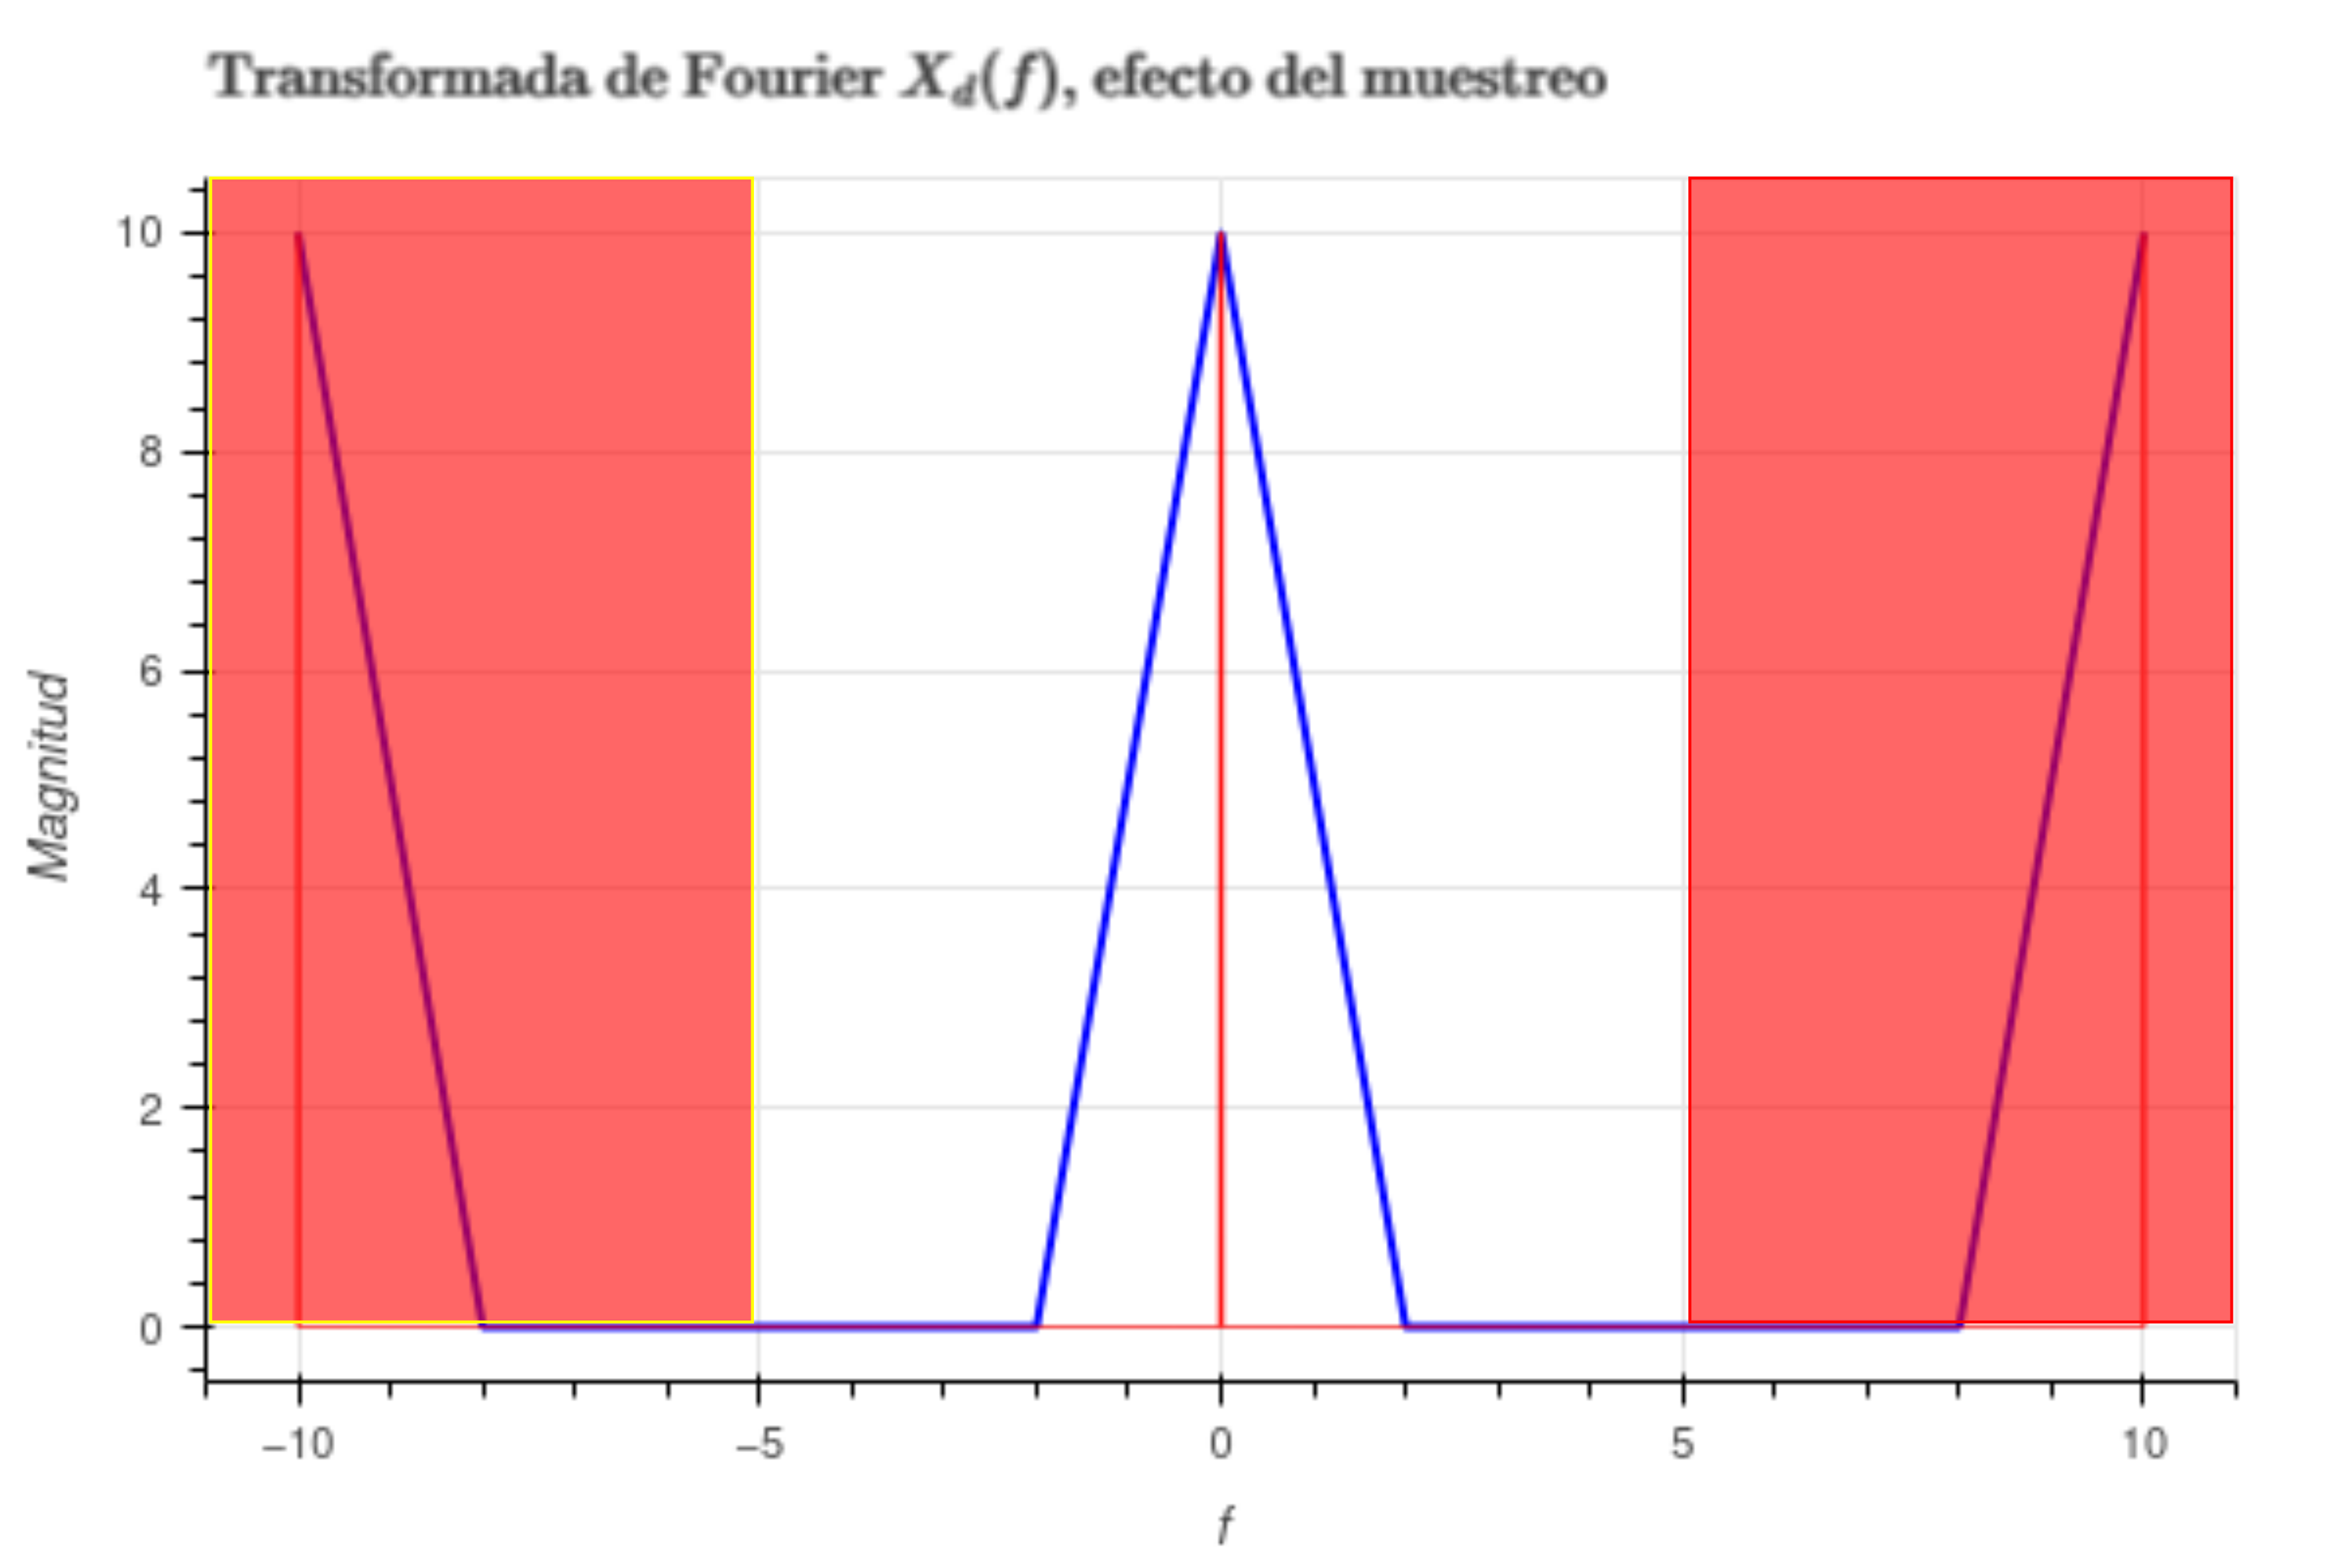
\includegraphics[width=5cm,clip,trim={0 0 0 22}]{Figures/reconstruccion_1.png}}
    \end{center}
    \begin{itemize}\scriptsize
      \item Recordemos que,
      \begin{itemize}\scriptsize
        \item $x_d(t)=\substack{\infty\\\sum\\n=-\infty}x[n]\delta(t-nT_s)$ 
        \item En frecuencia, el filtrado es $Y(\omega)=X_d(\omega)H(\omega)$.
        \item En el tiempo, $y(t)=\substack{\infty\\\int\\-\infty}x_d(\tau)h(t-\tau)d\tau$
      \end{itemize} 
    \end{itemize}
    \begin{alertblock}{Reconstrucción con retenedor ideal}\centering\scriptsize
      $\begin{aligned}
        y(t)&=\frac{\omega_c T_s}{\pi}\substack{\infty\\\sum\\n=-\infty}x_d[n] \text{sa}(\omega_c(t-nT_s)) \\
            &=2f_c T_s \substack{\infty\\\sum\\n=-\infty}x_d[n] \text{sinc}(2 f_c(t-nT_s)) 
      \end{aligned}$
    \end{alertblock}
  \end{frame}

  \begin{frame}\frametitle{Reconstrucción de señales}
    \begin{center}
      \alert {Reconstrucción ideal}\\
      \raisebox{-.5\height}{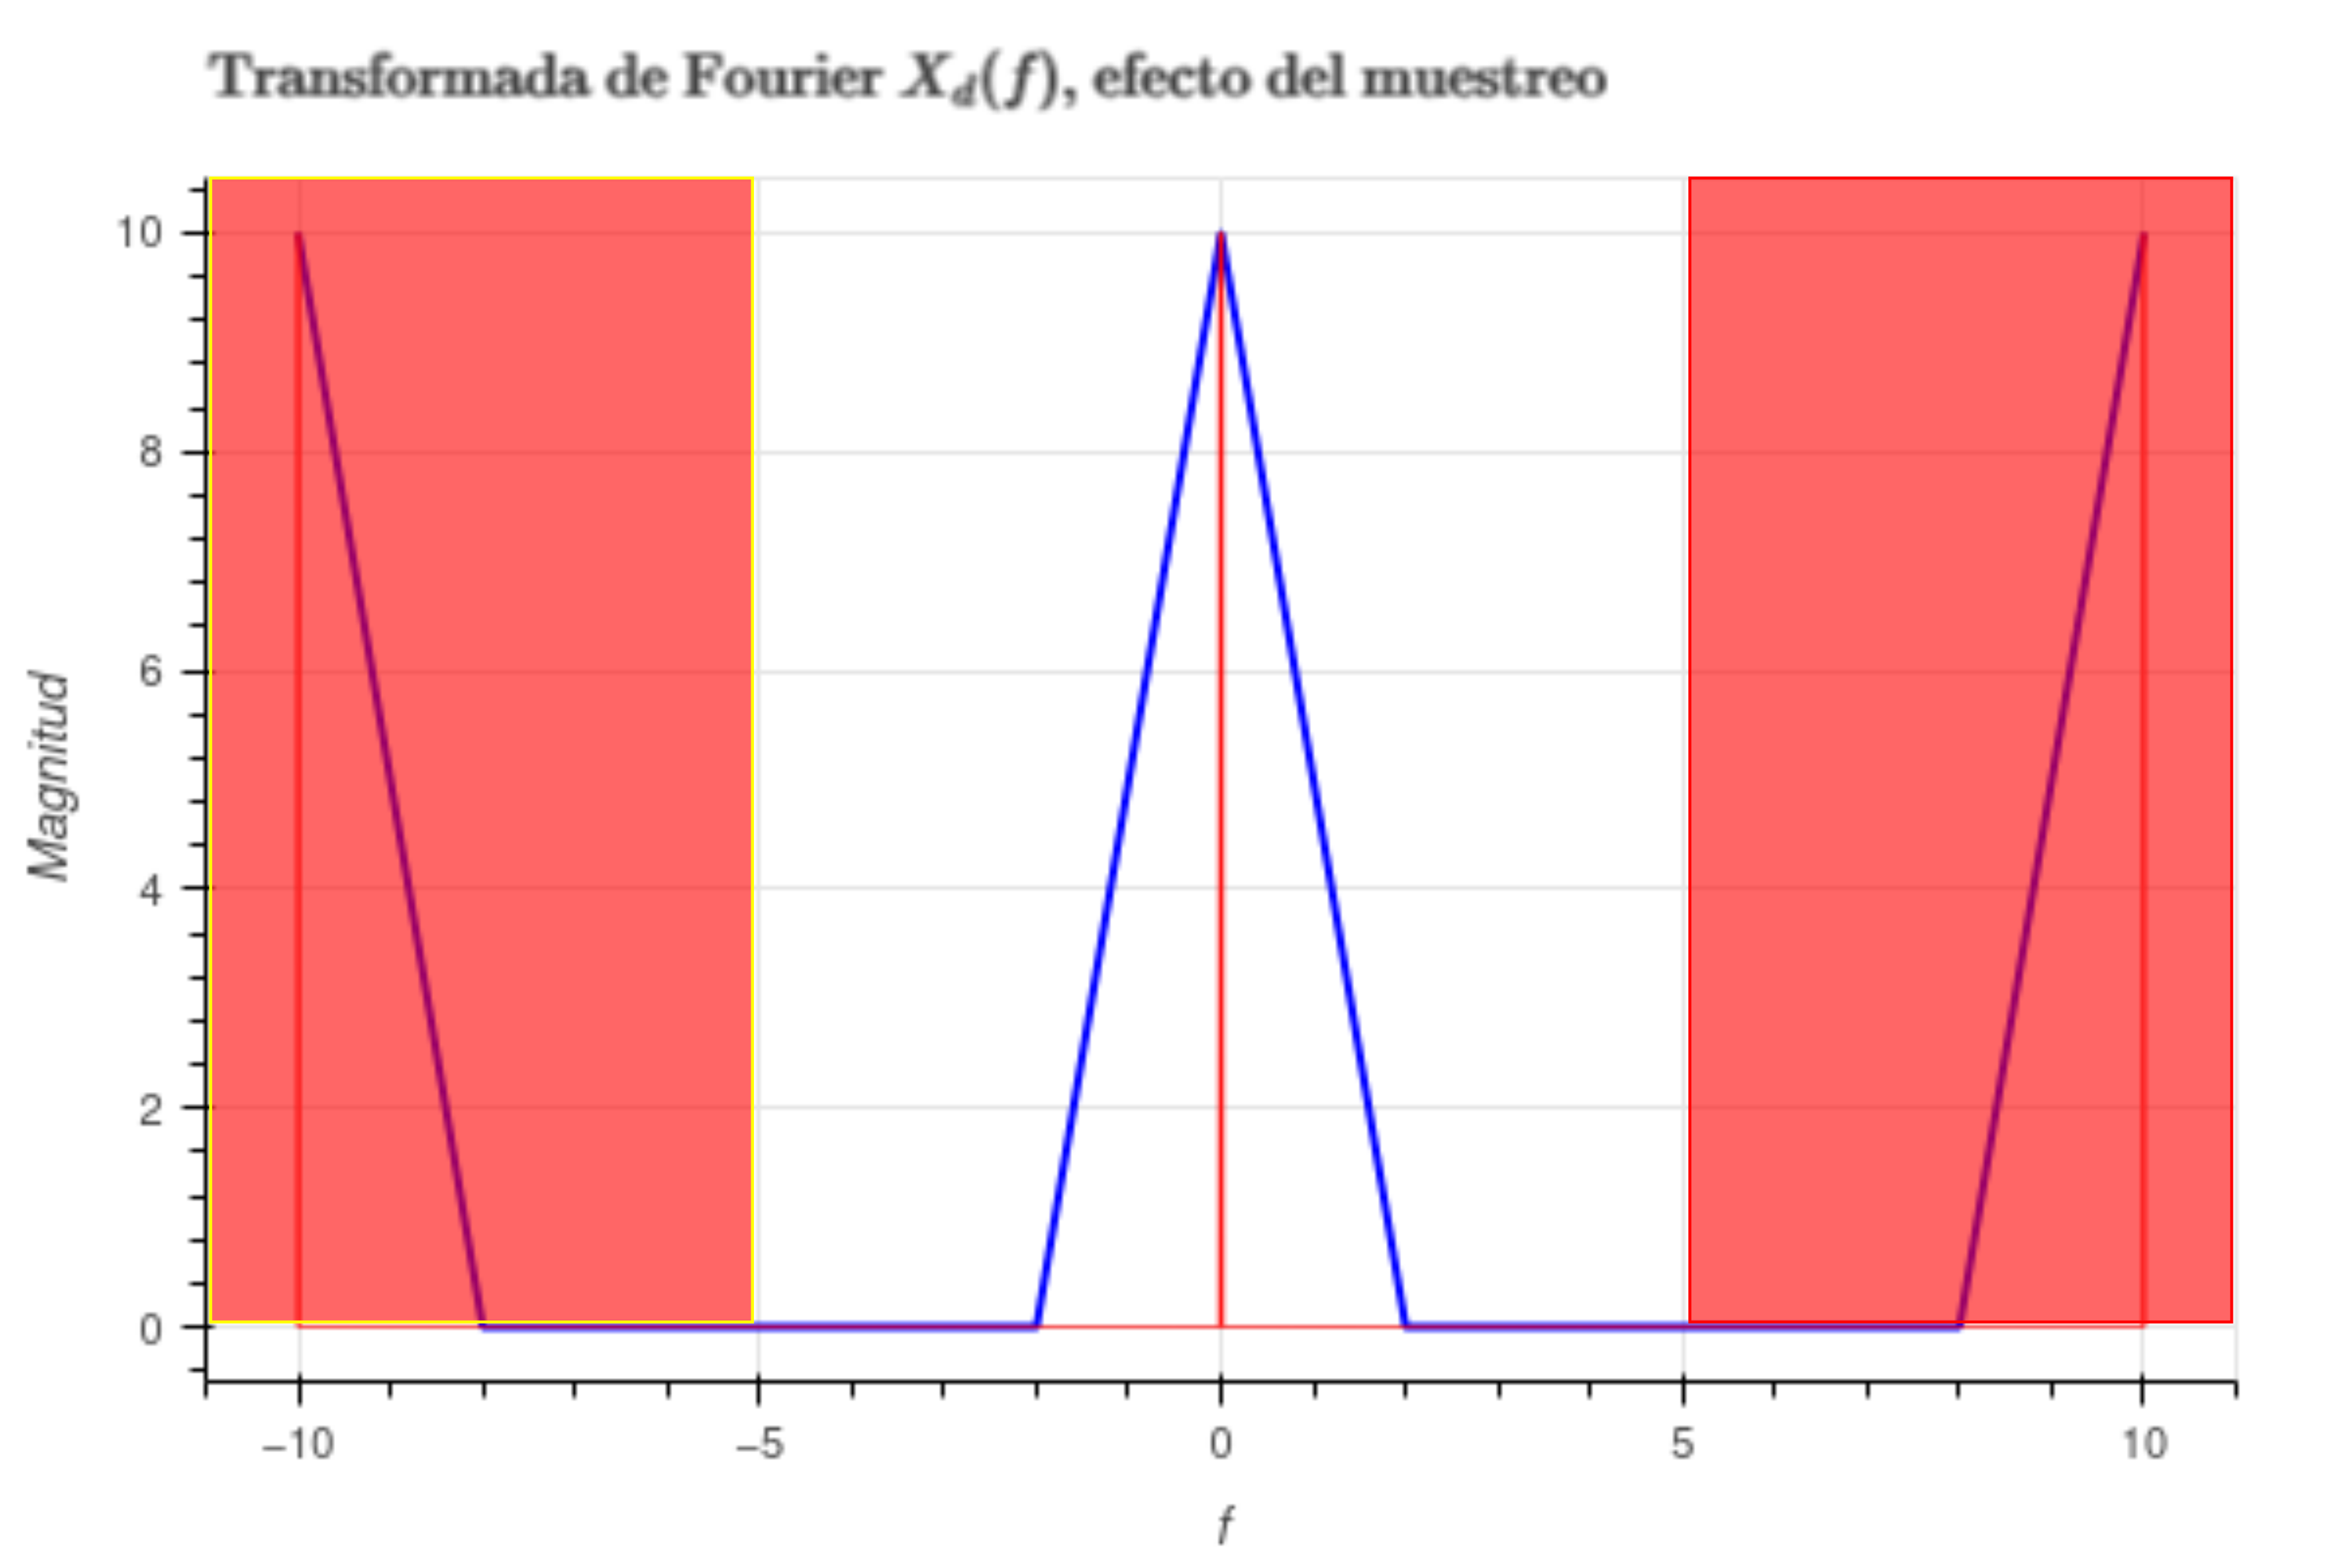
\includegraphics[width=5cm,clip,trim={0 0 0 22}]{Figures/reconstruccion_1.png}}
    \end{center}
    \begin{itemize}\scriptsize
      \item Algunas observaciones:
      \begin{itemize}\scriptsize
        \item Podemos elegir para $\omega_c$ cualquier valor en el rango $\omega_m<\omega_c<\omega_s - \omega_m$.
        \item Si elegimos $\omega_c=\frac{\omega_s}{2}$ la expresión se simplifica.
      \end{itemize} 
    \end{itemize}
    \begin{alertblock}{Reconstrucción con retenedor ideal}\centering
      $y(t)=\substack{\infty\\\sum\\n=-\infty}x_d[n] \text{sinc}(\frac{t-nT_s}{T_s})$
    \end{alertblock}
  \end{frame}

  \begin{frame}\frametitle{Reconstrucción por interpolación}
    \begin{center}
      \raisebox{-.5\height}{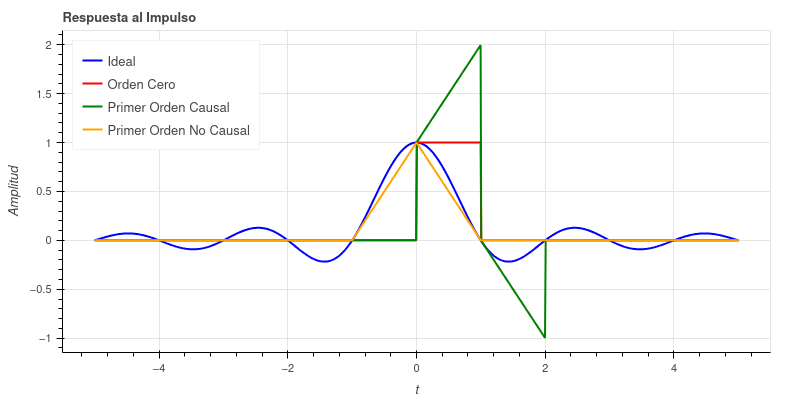
\includegraphics[width=5.5cm]{Figures/retenedor_t.png}}
      \raisebox{-.5\height}{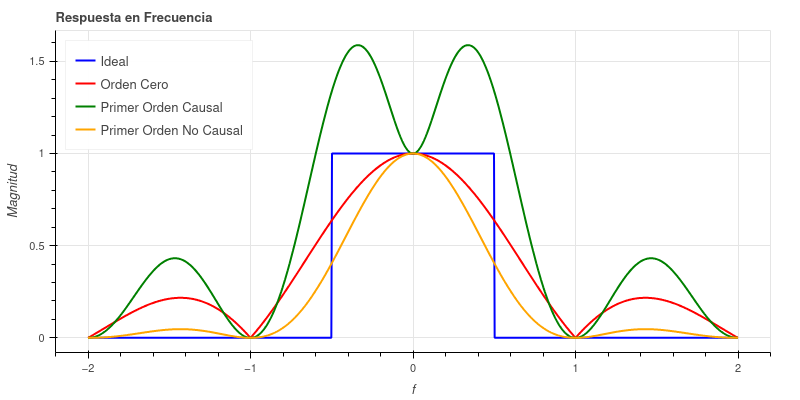
\includegraphics[width=5.5cm,clip,trim={0 0 0 25}]{Figures/retenedor_f.png}}
    \end{center}
    \begin{itemize}\scriptsize
      \item En general, podemos interpretar la reconstruccion como una interpolación.
      \begin{itemize}\scriptsize
        \item El valor de $x(t)$ se calcula a partir de las muestras.
        \item La función de interpolación $h(t)$ indica la contribución de las muestras al total.
        \item La contribución de cada muestra depende de la distancia al valor interpolado.
      \end{itemize} 
    \end{itemize}
    \begin{alertblock}{Reconstrucción con retenedor ideal}\centering
      $y(t)=\substack{\infty\\\sum\\n=-\infty}x_d[n] h(t-nT_s)$
    \end{alertblock}
  \end{frame}

  \begin{frame}\frametitle{Conceptos importantes}
    \begin{itemize}
      \item \alert{Teorema del muestreo}
      \begin{itemize}
        \item Escalado y réplica
        \item $\omega_s>2\omega_m$ (para evitar solapamiento)
      \end{itemize}
      \item \alert{Reconstrucción}
      \begin{itemize}
        \item Filtro paso-bajo ideal
        \item Interpolación
      \end{itemize}
    \end{itemize}
  \end{frame}
\end{document}
